\chapter{Pendahuluan}
\label{chap:pendahuluan}

\section{Latar Belakang}
\label{sec:latarbelakang}

KIRI adalah sebuah aplikasi yang membantu pengguna dalam menggunakan kendaraan umum \cite{statickiri}. Peran KIRI sangat sederhana, yaitu jika diberitahu di mana lokasi sekarang dan kemana lokasi tujuan, lalu KIRI akan memberitahu bagaimana cara sampai ke lokasi tujuan dengan menggunakan kendaraan umum. 

\begin{figure}[H]
	\centering
		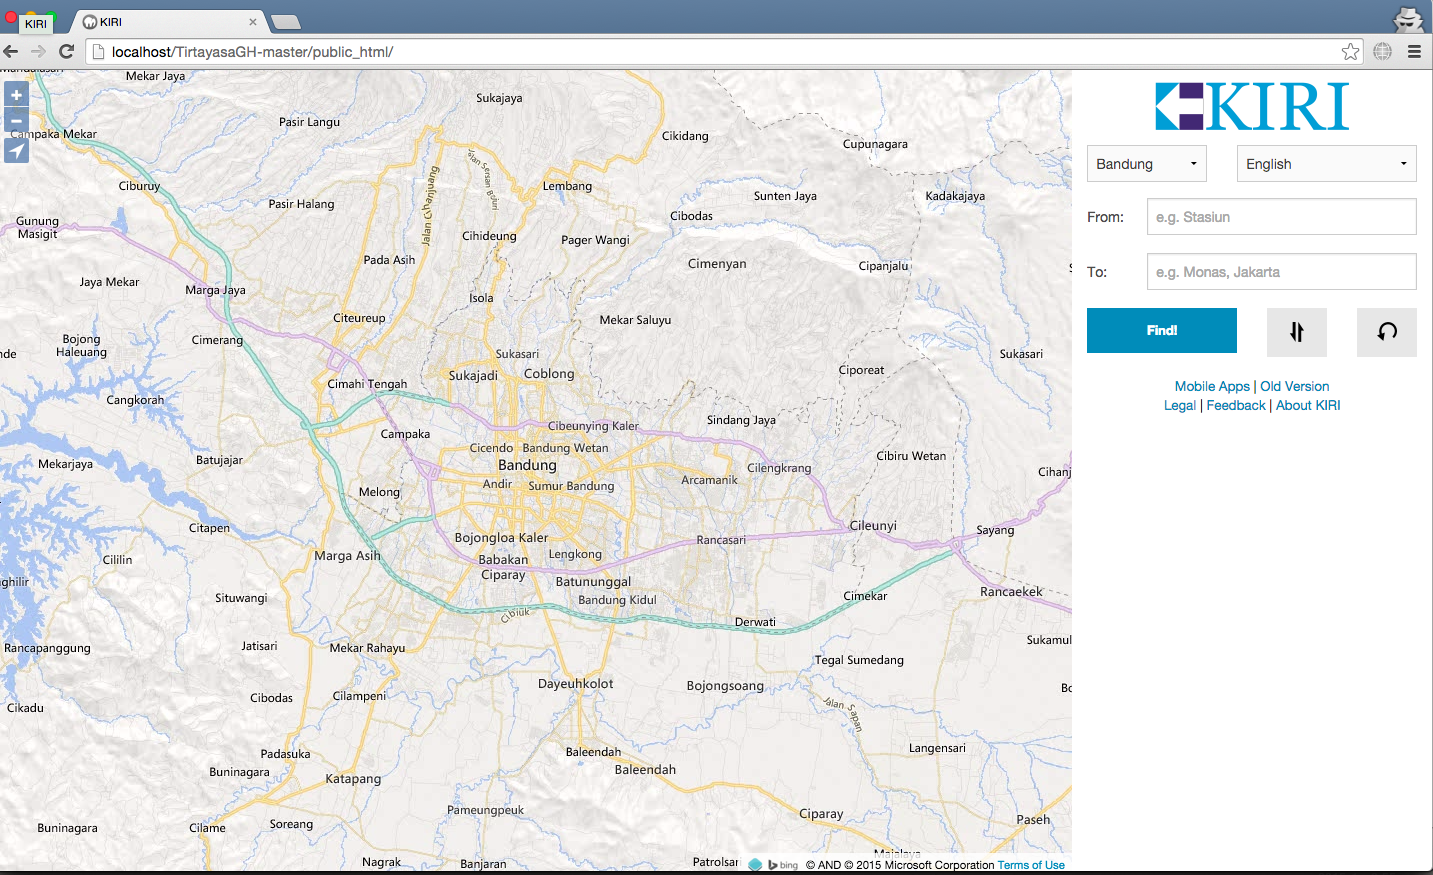
\includegraphics[scale=0.3]{Gambar/KIRI-main-5.png}
	\caption{Situs halaman web KIRI}
	\label{fig:1_kiritravel}
\end{figure}


Kode KIRI \cite{githubkiri} menggunakan bahasa PHP. Bahasa PHP merupakan bahasa \textit{scripting} yang cocok untuk pengembangan halaman \textit{web} \cite{phpnet}. Bahasa PHP tidak cocok untuk proyek besar. Masalah yang sering dijumpai pada bahasa PHP adalah tidak ada deklarasi tipe variabel. Tipe variabel pada PHP ditentukan pada saat \textit{runtime} tergantung pada konteks apa variabel tersebut digunakan. Hal ini memicu banyaknya kesalahan tipe data dalam aplikasi. Contoh masalahnya adalah jika terdapat 2 buah konstanta, konstanta pertama bertipe \textit{Integer} dan konstanta kedua bertipe \textit{String}, jika melakukan operasi penjumlahan antara konstanta pertama dan kedua tetap dapat dieksekusi dalam PHP, namun hasilnya tidak sesuai dengan yang diharapkan.

%\textit{Type safety} \footnote{ \url{https://en.wikipedia.org/wiki/Type_safety}, diakses 27 Oktober 2015} adalah fitur keamanan untuk mencegah kesalahan tipe data. Kesalahan tipe data dapat disebabkan oleh perbedaan tipe untuk konstanta program, variabel, dan fungsi. Sebagai contoh tipe data yang dibutuhkan berupa Float tetapi dalam program tipe data yang dimasukkan berupa Integer. Beberapa bahasa pemrograman terdapat fitur \textit{type safety}. Java mendukung Type Safety.
Bahasa pemrograman Java merupakan bahasa pemrograman yang \textit{statically-typed}, yang berarti semua varibel harus dideklarasikan terlebih dahulu sebelum digunakan \cite{java}. Tipe data variabel menentukan nilai yang dapat dimasukkan ke variabel tersebut dan operasi yang dapat dilakukan pada variabel tersebut. Dengan menggunakan Java, kesalahan tipe data dapat dicegah. Kesalahan tipe data dapat disebabkan oleh perbedaan tipe untuk konstanta program, variabel, dan fungsi.

\play adalah \textit{framework} untuk aplikasi web dengan menggunakan bahasa Java dan Scala. Bahasa Java dalam \play digunakan untuk struktur dan logika data, sedangkan bahasa Scala dalam \play digunakan untuk tampilan. \play mempunyai antarmuka yang sederhana, nyaman, fleksibel, dan kuat. \play menerapkan konsep arsitektur MVC, yaitu \textit{Model, View, Controller} \cite{playforjava}. Konsep arsitektur MVC memisahkan bagian struktur data \textit{Model} dan tampilan \textit{View} sehingga tidak mempunyai ketergantungan, sedangkan \textit{Controller} berfungsi untuk menghubungkan antara \textit{Model} dengan \textit{View}.

Pengembangan yang dilakukan adalah melakukan \textit{porting} kode KIRI yang dibuat dalam bahasa PHP menjadi bahasa Java dengan menggunakan \play tanpa mengurangi fungsi yang sudah ada sebelumnya.

\section{Rumusan Masalah}
\label{rumusanMasalah}
Rumusan masalah yang akan dibahas pada skripsi ini adalah:
\begin{enumerate}
	\item Bagaimana memahami dan menganalisis kode KIRI \textit{Front-End Server Side} dalam bahasa PHP?
	\item Bagaimana melakukan porting kode KIRI \textit{Front-End Server Side} dalam bahasa PHP menjadi Play Framework (Java) ?
	\item Bagaimana perbandingan waktu eksekusi antara KIRI \textit{Front-End Server Side} yang dibangun dengan PHP dan KIRI \textit{Front-End Server Side} yang dibangun dengan bahasa Java?
\end{enumerate}

\section{Tujuan}
\label{sec:tujuan}
Berdasarkan rumusan masalah yang telah dibuat, maka tujuan penelitian ini dijelaskan ke dalam poin-poin sebagai berikut:
\begin{enumerate}
	\item Memahami dan menganalisis kode KIRI \textit{Front-End Server Side}.
	\item Melakukan porting kode KIRI \textit{Front-End Server Side} dalam bahasa PHP menjadi Play Framework (Java).
	\item Membandingkan waktu eksekusi antara KIRI \textit{Front-End Server Side} yang dibangun dengan PHP dan KIRI \textit{Front-End Server Side} yang dibangun dengan bahasa Java.
\end{enumerate}

\section{Batasan Masalah}
\label{sec:batasanMasalah}
Beberapa batasan dengan skripsi ini adalah:
\begin{enumerate}
	\item Play Framework yang digunakan adalah versi 2.4.3.
	\item Kode KIRI yang digunakan adalah versi commit \verb!`b650bfa'! yang tersedia di Github pascalalfadian\cite{githubkiri}.
	%\item URL \url{http://newmenjangan.cloudapp.net:8000} dan \url{https://angkot.web.id} online.
\end{enumerate}

\section{Metode Penelitian}
\label{sec:metodePenelitian}
Berikut adalah metode penelitian yang digunakan dalam pembuatan skripsi ini:
	\begin{enumerate}
		\item Melakukan studi literatur tentang metode yang berkaitan dengan kode KIRI \textit{Front-End Server Side}, Play Framework, JDBC, dan JSON.
		\item Memahami dan melakukan analisis kode KIRI \textit{Front-End} serta teori-teori untuk membangun KIRI \textit{Front-End Server Side} dalam bahasa Java menggunakan Play Framework.
		\item Merancang dan mengimplementasikan kode KIRI \textit{Front-End Server Side} menjadi bahasa Java menggunakan Play Framework.
		\item Melakukan pengujian dan eksperimen.
		\item Membuat dokumen skripsi.
	\end{enumerate}
	
\section{Sistematika Penulisan}
\label{sec:sistematikaPenulisan}
Setiap bab dalam penelitian ini memiliki sistematika penulisan yang dijelaskan sebagai berikut:
	\begin{enumerate}
		\item Bab 1: Pendahuluan, yaitu membahas gambaran umum dari penelitian, yaitu tentang latar belakang, rumusan masalah, tujuan, batasan masalah, metode penelitian dan sistematika penulisan.
		\item Bab 2: Dasar Teori, yaitu membahas mengenai teori-teori yang mendukung berjalannya skripsi ini yang berisi tentang penggunaan Play Framework, JDBC, dan JSON.
		\item Bab 3: Analisis, yaitu membahas mengenai analisis masalah yang berisi tentang kode KIRI \textit{Front-End Server Side} saat ini, analisis antarmuka saat ini, analisis sistem usulan.
	\item Bab 4: Perancangan, yaitu membahas mengenai perancangan yang dilakukan sebelum melakukan implementasi meliputi diagram kelas rinci beserta deskripsi kelas dan fungsinya dan perancangan antarmuka usulan.
	\item Bab 5: Implementasi dan Pengujian, yaitu membahas mengenai implementasi dan pengujian aplikasi, meliputi lingkungan implementasi, hasil implementasi, pengujian fungsional, dan pengujian eksperimental.
	\item Bab 6: Kesimpulan dan Saran, yaitu berisi kesimpulan dari hasil pembangunan aplikasi beserta saran untuk pengembangan selanjutnya.
	\end{enumerate}
		